\chapter{The Software Heritage Property Graph Dataset}%
\label{chp:graph-dataset}

This chapter is based on an article~\cite{swh-msr2019-dataset} accepted at the
16th International Conference on Mining Software Repositories (MSR 2019), and
the presentation~\cite{msr-2020-challenge} for its subsequent use as the
``Mining Challenge'' of the 17th International Conference on Mining Software
Repositories (MSR 2020).

\section{Introduction}

Up to this point, we have proposed ways to make the Software Heritage corpus
available to software mining studies of medium scale, up to tens of thousands
of repositories, either by retrieving bundles of related software artifacts
(\cref{chp:vault}) or by accessing the content remotely through a
virtual filesystem (\cref{chp:fuse}). Ultimately, our goal is to enable
\emph{universal software mining}, i.e., making it feasible for researchers to
study the \emph{entire corpus of software commons} for all the reasons
described in \cref{sec:universal-software-mining}. Notably, exhaustive
approaches are virtually the only way to get a realistic high-level picture of
the complex social networks and processes governing software development.

The main object of interest to study these strongly entangled and dynamic
relationships is the \emph{property
graph}~\cite{angles2018propertygraph,bonifati2018graphquery} of public software
development, i.e., the graph containing all the software artifacts in our
corpus, from the development history down to the source code trees and
individual blobs, along with all their associated properties.

Exhaustive studies of the source code files themselves are very expensive, both
in terms of required storage space and bandwidth to fetch the entirety of more
than 10 billion blobs totaling around 850\,TiB of storage space as of May
2021, and in terms of computing power to process this vast amount of data.
However, the property graph of software development \emph{excluding the blobs
themselves} is in itself a valuable trove of data, while only being a fraction
of that size.  It notably contains all the directory and file hierarchies of
the source code, its entire development history and all associated metadata,
including authorship graphs.

By making the property graph easy to analyze in an exhaustive manner, we can
significantly advance towards our goal of universal software mining on several
fronts. The immediate benefit is to enable studies that aim to analyze the
underlying development processes and social communities in the software
commons, as they generally do not need access to the blobs themselves since the
network relationships are directly present in the graph. More broadly, it also
helps mining studies that do analyze source code by allowing researchers to
precisely narrow the set of source code files they need prior to actually
fetching them, in order to minimize bandwidth and storage requirements.

In this chapter we introduce the \emph{Software Heritage Property Graph
Dataset}, a corpus of all development artifacts archived by \SWH{} made freely
available for research in both a graph representation and a relational format
suitable for scale-out analysis.
While this dataset excludes source code blobs, it does include their
cryptographic checksums, which can be used to retrieve the actual files from
any \SWH{} mirror using a Web
API\footnote{\url{https://archive.softwareheritage.org/api/}} and
cross-reference files encountered in the wild, including in other datasets.

\subsection{Related Work}%
\label{sec:graph-dataset-related}

To the best of our knowledge, no existing public dataset contains a comparable
amount and diversity of data about source code artifacts extracted from public
software development.

The Debsources dataset~\cite{debsources-ese-2016} contains a wealth of
information about Debian releases over several decades, but stops at the
release granularity (rather than commits) and is at least three orders of
magnitude smaller than the present dataset.

GHTorrent~\cite{GHTorrent} covers GitHub and includes
non-source-code artifacts (e.g., issues, pull requests, etc.), but lacks
software hosted in other locations (e.g., GitLab, Debian, PyPI).
Also, no deduplication applies to GHTorrent, making cloning tracking more
challenging.
The GitHub Activity Data~\cite{web:github-activity-data} dataset is similar to
GHTorrent, but contains less metadata; it can be directly queried in the
Google BigQuery cloud platform using relational query languages.
CodeFeedr~\cite{DBLP:conf/icse/VargasHKBG18} is a natural evolution of
GHTorrent, but it is oriented toward expanding coverage for additional sources
of non-source-code artifacts.

World of Code (WoC)~\cite{mockus2019woc} is a recent attempt at providing a
corpus for large-scale VCS analyses, with a target scale similar to ours (18
billion objects as of October 2020). However, the sourcing diversity of the
dataset is more limited, only covering Git and GitHub and excluding other
\glspl{VCS} and hosting locations.

\section{Relational model}%
\label{sec:relational-model}

The most common pattern in distributed big data analysis is to query datasets
provided in a \emph{relational format}, i.e., as a set of data tables linked
together by predefined relationships. The relational \emph{schema} describes
these tables, notably the types of their individual columns and the way they
relate to each other. These data tables can then be loaded in distributed Big
Data engines and queried using relational query languages like SQL\@.

The data in the Software Heritage archive is already internally stored in a
relational format inside a PostgreSQL database. However, this format is
optimized for different constraints, notably shrinking disk space usage at the
expense of speed by \emph{normalizing} tables (i.e., reducing data redundancy
as much as possible). While this trade-off is acceptable for long-term storage,
it requires more expensive ``join'' operations to combine tables together,
which is generally undesirable for scale-out processing as it adds more
synchronization points between the different shards. Instead, when using
distributed Big Data engines it is more efficient to \emph{denormalize} the
data: using larger tables which increases redundancy while reducing the need
for join operations.

\begin{figure}
    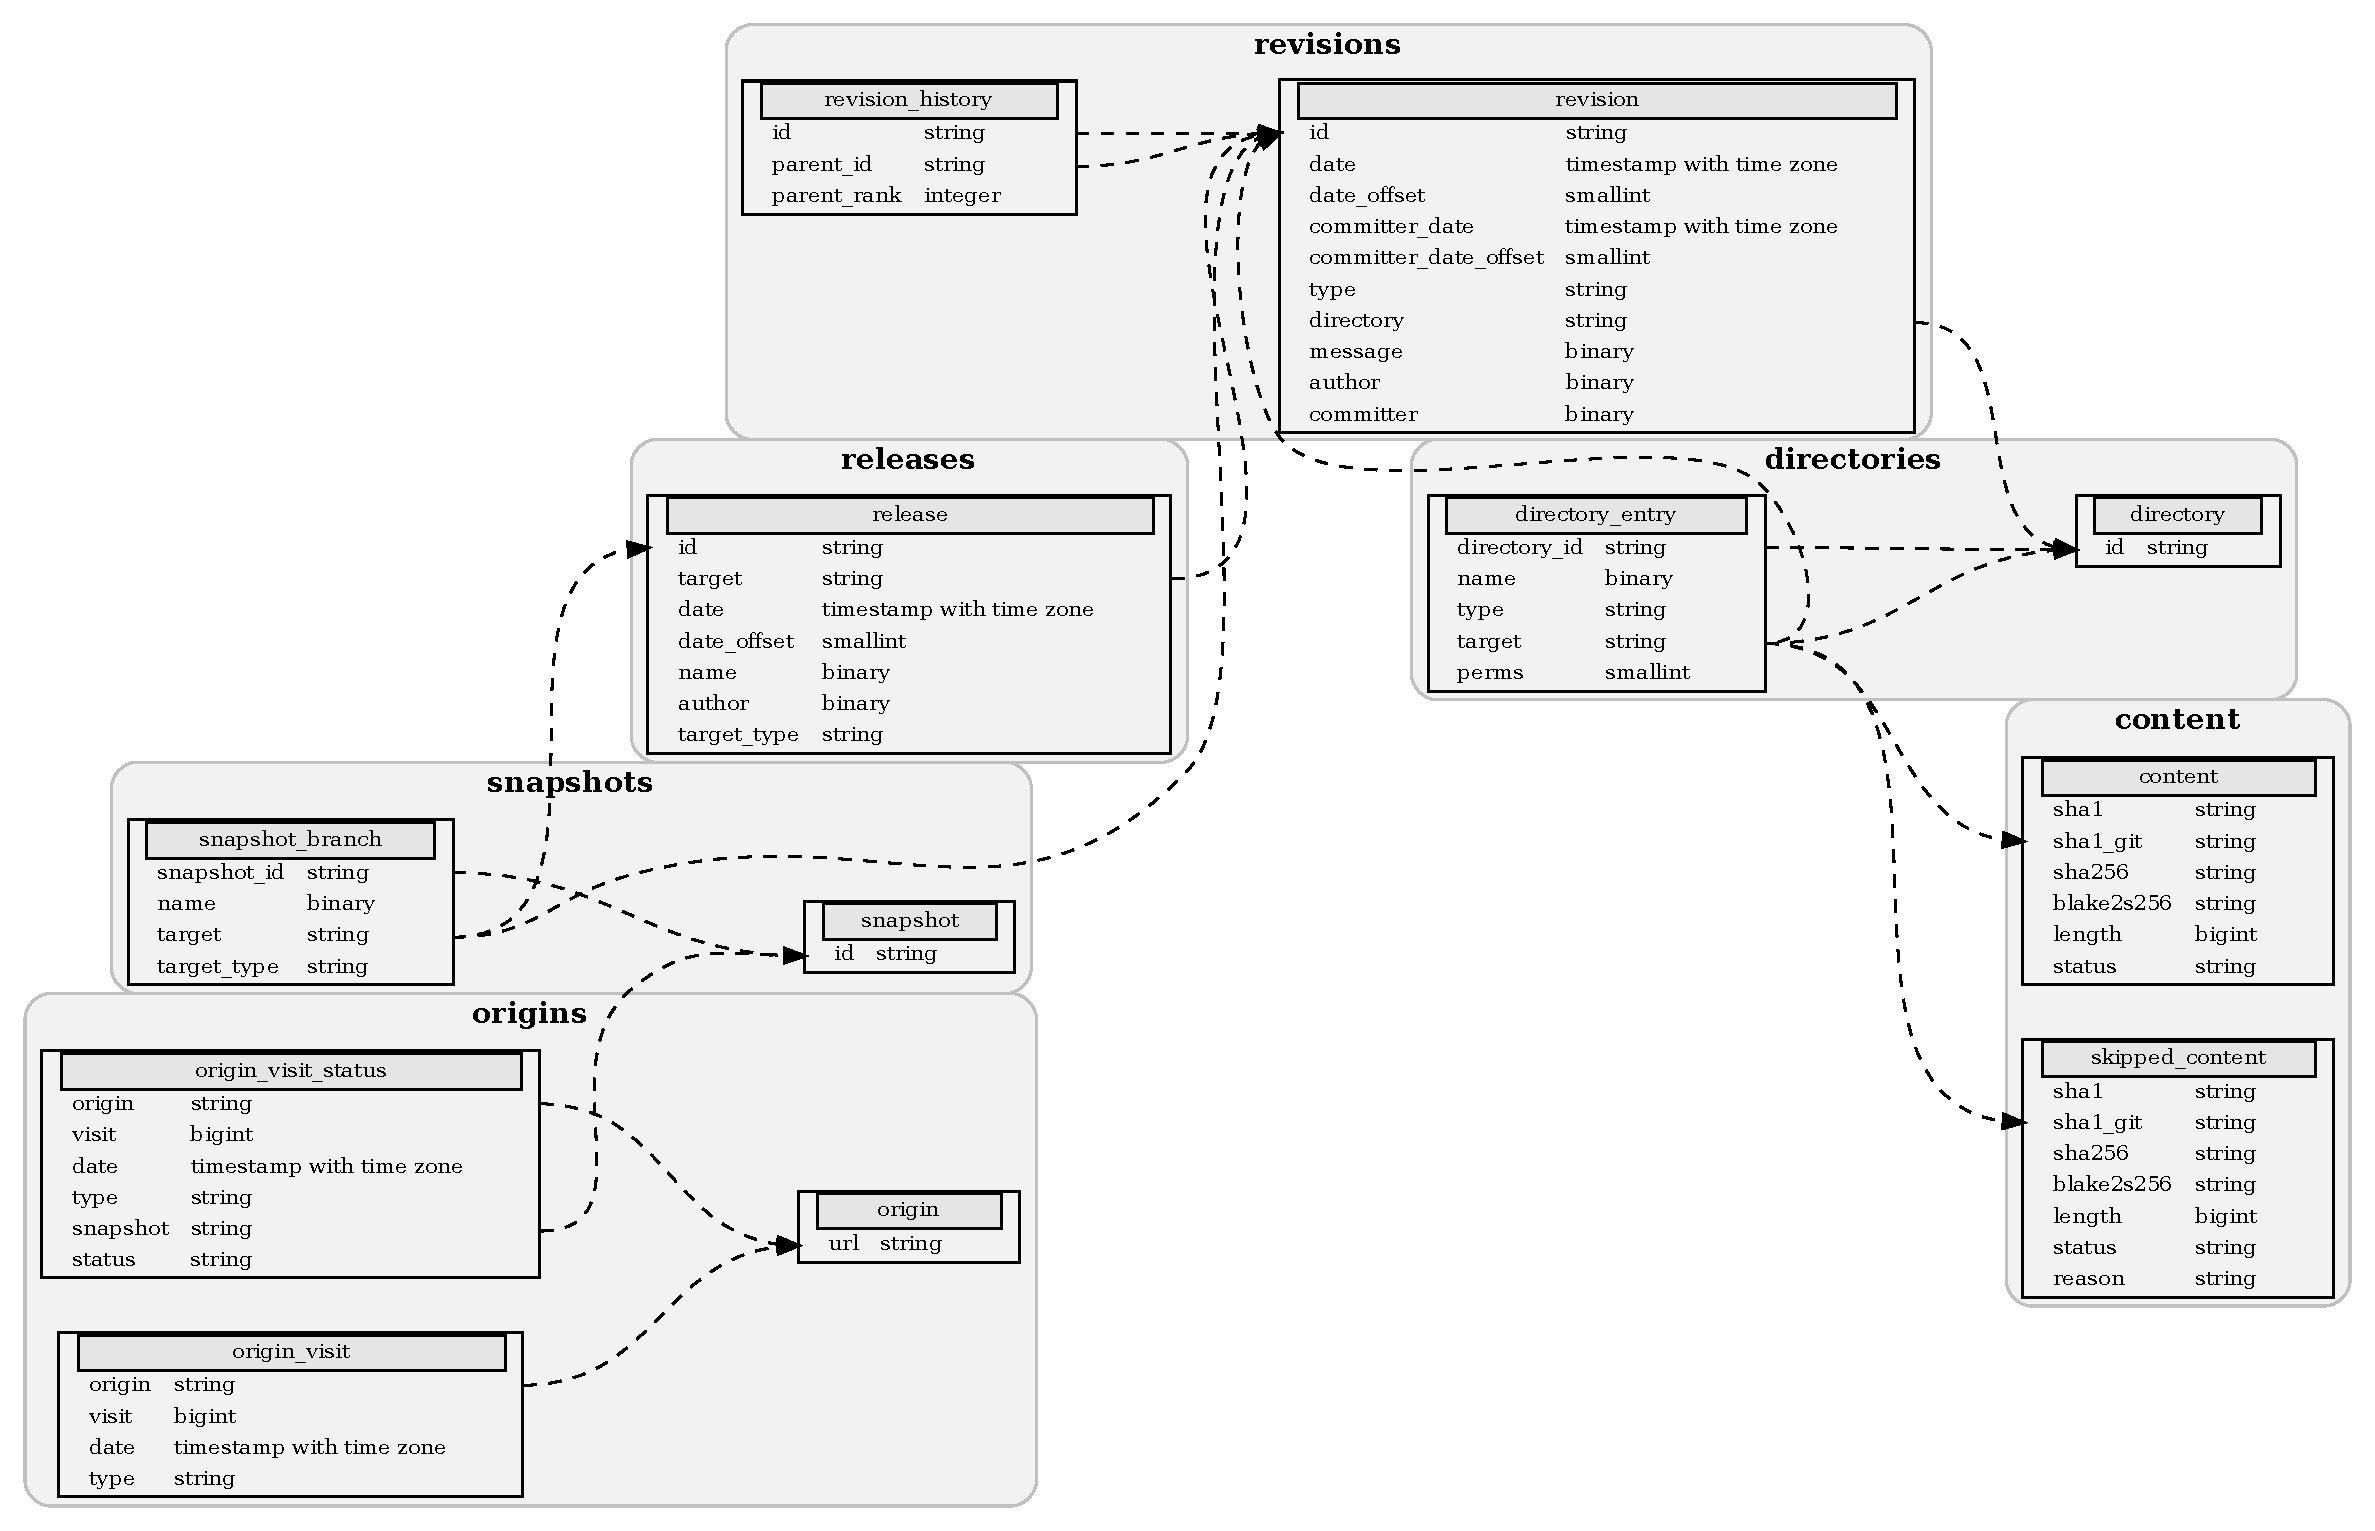
\includegraphics[width=\linewidth]{img/graph-dataset/db-schema}
    \caption{Relational schema of the \SWHGD{}.}%
    \label{fig:swh-dataset-schema}
\end{figure}

\Cref{fig:swh-dataset-schema} presents the relational schema of the \SWHGD{}.
It significantly differs from the original schema of the PostgreSQL
storage\footnote{\url{https://docs.softwareheritage.org/devel/swh-storage/sql-storage.html}}
in a few ways. In the latter, the directory table is normalized to avoid storing
redundant copies of hashes by using an array of directory entries. After some
experimentation on various cloud services, we determined that arrays of
arbitrary length in distributed Big Data engines are a performance killer, as
they hinder the ability of the query planner to properly shard computations
among a right-sized pool of nodes by making the size of each row hard to
predict. Some cloud services like Google BigQuery have size limits on arrays,
which makes it impossible to store directories of arbitrary length. We
denormalized that table, as well as two of the snapshot tables. Another minor
change is the use of hexadecimal string representation of intrinsic hashes
instead of binary strings, as developers tend to be more comfortable using
this hexadecimal representation directly. Finally, some columns which we
considered to be mostly implementation details that would not be useful for
data analysis were removed from the schema.

\paragraph*{Anonymization and ethical considerations.}
Because the dataset is intended to be distributed to a wide audience,
particular attention needs to be paid to the \gls{PII} contained in the graph,
namely the names and e-mail addresses of revision authors. Because this
personal data has been shared by subjects publicly, storing and sharing this
data on an opt-out basis complies with data protection laws. However, this
poses some ethical concerns, as making this data easy to access and process
also makes these commit authors more susceptible to potential abuse, like
e-mail spam. This is not a new problem, and has notably been encountered by
Gousios in the GHTorrent project~\cite{gousios2016issue32}.

Our approach to deal with these ethical considerations is two-fold. First, we
anonymize all the data provided in the dataset by running a cryptographic hash
on the names and e-mail addresses; if needed, they can be individually
requested from the archive API using the commit identifiers, although this
access is subject to the usual API quotas. Further, we make access to the
dataset conditional on the acceptance of an Ethical
Charter\footnote{\url{https://www.softwareheritage.org/legal/users-ethical-charter/}}
and specific terms of use for bulk
access\footnote{\url{https://www.softwareheritage.org/legal/bulk-access-terms-of-use/}}.

This anonymization process does not hinder the possibility of relating together
commits which have the same author, which is an important need in many research
use cases. Because cryptographic hashing is both one-way and deterministic, it
is possible to check whether two commits have the same author by comparing the
resulting hashes, without being able to reverse the original author name.

\paragraph*{Schema.}
The tables in the relational schema of the Software Heritage Graph Dataset are
defined as follows:


\begin{itemize}
\item
  \textbf{content}: contains information on the blobs (source file contents) stored in the
  archive.

  \begin{itemize}
  \tightlist
  \item
    \texttt{sha1} (string): the SHA-1 of the content (hexadecimal)
  \item
    \texttt{sha1\_git} (string): the Git SHA-1 of the content
    (hexadecimal)
  \item
    \texttt{sha256} (string): the SHA-256 of the content (hexadecimal)
  \item
    \texttt{blake2s256} (bytes): the BLAKE2s-256 of the content
    (hexadecimal)
  \item
    \texttt{length} (integer): the length of the content
  \item
    \texttt{status} (string): the visibility status of the content
  \end{itemize}
\item
  \textbf{skipped\_content}: contains information on the contents that
  were encountered in the wild but not archived for various reasons.

  \begin{itemize}
  \tightlist
  \item
    \texttt{sha1} (string): the SHA-1 of the skipped content
    (hexadecimal)
  \item
    \texttt{sha1\_git} (string): the Git SHA-1 of the skipped content
    (hexadecimal)
  \item
    \texttt{sha256} (string): the SHA-256 of the skipped content
    (hexadecimal)
  \item
    \texttt{blake2s256} (bytes): the BLAKE2s-256 of the skipped content
    (hexadecimal)
  \item
    \texttt{length} (integer): the length of the skipped content
  \item
    \texttt{status} (string): the visibility status of the skipped
    content
  \item
    \texttt{reason} (string): the reason why the content was skipped
  \end{itemize}
\item
  \textbf{directory}: contains the directories stored in the archive.

  \begin{itemize}
  \tightlist
  \item
    \texttt{id} (string): the intrinsic hash of the directory
    (hexadecimal), recursively computed with the Git SHA-1 algorithm
  \end{itemize}
\item
  \textbf{directory\_entry}: contains the entries in directories.

  \begin{itemize}
  \tightlist
  \item
    \texttt{directory\_id} (string): the Git SHA-1 of the directory
    containing the entry (hexadecimal).
  \item
    \texttt{name} (bytes): the name of the file (basename of its path)
  \item
    \texttt{type} (string): the type of object the branch points to
    (either \texttt{revision}, \texttt{directory} or \texttt{content}).
  \item
    \texttt{target} (string): the Git SHA-1 of the object this entry
    points to (hexadecimal).
  \item
    \texttt{perms} (integer): the permissions of the object
  \end{itemize}
\item
  \textbf{revision}: contains the revisions stored in the archive.

  \begin{itemize}
  \tightlist
  \item
    \texttt{id} (string): the intrinsic hash of the revision
    (hexadecimal), recursively computed with the Git SHA-1 algorithm.
    For Git repositories, this corresponds to the commit hash.
  \item
    \texttt{message} (bytes): the revision message
  \item
    \texttt{author} (string): an anonymized hash of the author of the
    revision.
  \item
    \texttt{date} (timestamp): the date the revision was authored
  \item
    \texttt{date\_offset} (integer): the offset of the timezone of
    \texttt{date}
  \item
    \texttt{committer} (string): an anonymized hash of the committer of
    the revision.
  \item
    \texttt{committer\_date} (timestamp): the date the revision was
    committed
  \item
    \texttt{committer\_date\_offset} (integer): the offset of the
    timezone of \texttt{committer\_date}
  \item
    \texttt{directory} (string): the Git SHA-1 of the directory the
    revision points to (hexadecimal). Every revision points to the root
    directory of the project source tree to which it corresponds.
  \end{itemize}
\item
  \textbf{revision\_history}: contains the ordered set of parents of
  each revision. Each revision has an ordered set of parents (0 for the
  initial commit of a repository, 1 for a regular commit, 2 for a
  regular merge commit and 3 or more for octopus-style merge commits).

  \begin{itemize}
  \tightlist
  \item
    \texttt{id} (string): the Git SHA-1 identifier of the revision
    (hexadecimal)
  \item
    \texttt{parent\_id} (string): the Git SHA-1 identifier of the parent
    (hexadecimal)
  \item
    \texttt{parent\_rank} (integer): the rank of the parent, which
    defines the ordering between the parents of the revision
  \end{itemize}
\item
  \textbf{release}: contains the releases stored in the archive.

  \begin{itemize}
  \tightlist
  \item
    \texttt{id} (string): the intrinsic hash of the release
    (hexadecimal), recursively computed with the Git SHA-1 algorithm
  \item
    \texttt{target} (string): the Git SHA-1 of the object the release
    points to (hexadecimal)
  \item
    \texttt{date} (timestamp): the date the release was created
  \item
    \texttt{author} (integer): the author of the revision
  \item
    \texttt{name} (bytes): the release name
  \item
    \texttt{message} (bytes): the release message
  \end{itemize}
\item
  \textbf{snapshot}: contains the list of \gls{VCS} snapshots stored in the
  archive.

  \begin{itemize}
  \tightlist
  \item
    \texttt{id} (string): the intrinsic hash of the snapshot
    (hexadecimal), recursively computed with the Git SHA-1 algorithm.
  \end{itemize}
\item
  \textbf{snapshot\_branch}: contains the list of branches associated
  with each snapshot.

  \begin{itemize}
  \tightlist
  \item
    \texttt{snapshot\_id} (string): the intrinsic hash of the snapshot
    (hexadecimal)
  \item
    \texttt{name} (bytes): the name of the branch
  \item
    \texttt{target} (string): the intrinsic hash of the object the
    branch points to (hexadecimal)
  \item
    \texttt{target\_type} (string): the type of object the branch points
    to (either \texttt{release}, \texttt{revision}, \texttt{directory}
    or \texttt{content}).
  \end{itemize}
\item
  \textbf{origin}: the software origins from which the projects in the
  dataset were archived.

  \begin{itemize}
  \tightlist
  \item
    \texttt{url} (bytes): the URL of the origin
  \end{itemize}
\item
  \textbf{origin\_visit}: the different visits of each origin. Since
  Software Heritage archives software continuously, software origins are
  crawled more than once. Each of these ``visits'' is an entry in this
  table.

  \begin{itemize}
  \tightlist
  \item
    \texttt{origin}: (string) the URL of the origin visited
  \item
    \texttt{visit}: (integer) an integer identifier of the visit
  \item
    \texttt{date}: (timestamp) the date at which the origin was visited
  \item
    \texttt{type} (string): the type of origin visited (e.g.,
    \texttt{git}, \texttt{pypi}, \texttt{hg}, \texttt{svn},
    \texttt{git}, \texttt{ftp}, \texttt{deb}, \ldots)
  \end{itemize}
\item
  \textbf{origin\_visit\_status}: the status of each visit.

  \begin{itemize}
  \tightlist
  \item
    \texttt{origin}: (string) the URL of the origin visited
  \item
    \texttt{visit}: (integer) an integer identifier of the visit
  \item
    \texttt{date}: (timestamp) the date at which the origin was visited
  \item
    \texttt{type} (string): the type of origin visited (e.g.,
    \texttt{git}, \texttt{pypi}, \texttt{hg}, \texttt{svn},
    \texttt{git}, \texttt{ftp}, \texttt{deb}, \ldots)
  \item
    \texttt{snapshot\_id} (string): the intrinsic hash of the snapshot
    archived in this visit (hexadecimal).
  \item
    \texttt{status} (string): the integer identifier of the snapshot
    archived in this visit, either \texttt{partial} for partial visits
    or \texttt{full} for full visits.
  \end{itemize}
\end{itemize}


\section{Dataset export pipeline}

\subsection{Point-in-time exports}

The dataset is exported from the \texttt{swh-journal} component of the archive,
which provides a log of all objects inserted in the archive, and is backed
by Apache Kafka as described in \cref{sec:swh-infrastructure}. While the
journal exposes a continuous stream of data, the property graph dataset is
intended to be a periodic dump in which the entire state of the graph is
exported at a given point in time.

Making periodic exports is generally easier for researchers, as they can
simply download the latest export without having to continuously synchronize
their own data with the archive using a mirroring protocol. This kind of
analysis on ``offline'' data is often the preferred way to run experiments on
one's own infrastructure. This is also useful for study repeatability, as the
date of the export can uniquely identify its content, whereas it would be
harder to reproduce the exact state of a continuously updating dataset at a
given date.

The journal is divided in ``topics'', one for each object type described
in \cref{sec:swh-artifacts}. The process exports each object type one by
one, in a sequential fashion. These topics are ordered so that objects at the
top of the graph are always exported first and those at the bottom exported
last (in order: origins, snapshots, releases, revisions, directories,
contents). This order uses the directionality of the graph to reduce the number
of ``dangling'' objects (i.e., objects that refer to objects not present in the
graph) at the cost of having more ``loose'' objects (i.e., objects that are not
referred to by any other objects). If the upper layers were exported last, they
would refer to newer objects in the journal that would have not been exported
before; exporting them first ensures that they refer to objects that will be
exported in the next steps.

\subsection{Parallelism}

Kafka achieves streaming scalability by dividing each topic into a certain
number of partitions that can be processed independently on the client side.
When new data is sent to the journal, each object is assigned to a partition
deterministically using its intrinsic hash.

Before exporting a topic, the current \emph{offsets} of each partition of that
topic are retrieved; they constitute the ``boundaries'' from and to which the
journal will be read. This ensures that the stream reader can terminate at a
fixed point, instead of trying to catch up with the live state of the journal.

A parallelism factor can be given on the command line of the exporter as
follows:

\begin{minted}{console}
$ swh dataset graph export --processes 64 output_dir/
\end{minted}

The partitions are split equally among each subprocess, which then start to
process them until they reach the high offset. Periodically, these subprocesses
report their current progress in the stream to a single process which
aggregates them and displays in real time the total progress in the queue.

\subsection{Resumability}

A dataset export can be attributed a unique export identifier that is passed
to the command line:

\begin{minted}{console}
$ swh dataset graph export --export-id dataset-2021-03-23 output_dir/
\end{minted}

This identifier is stored on the server side to associate the journal clients
with a given export.
When a batch of objects has been read from the journal, the client
automatically acknowledges to the server that they have correctly been
processed. The server maintains the last offset that has been acknowledged, or
``committed'', for each partition.
If an export is interrupted because of an error or a server failure, resuming
it can be achieved by reusing the same export identifier. The journal client
will then start reading the log after the last committed offset.

\subsection{Object unicity}%
\label{sec:dataset-export-unicity}

To guarantee that each object is only present once in the final export, there
needs to be a way to check whether a given object has already been exported in
case it appears multiple times in the log. The message delivery
semantics\footnote{\url{https://kafka.apache.org/documentation/\#semantics}} in
\texttt{swh-journal} are ``at least once'', which means that objects are
guaranteed to be present in the stream but might be delivered multiple times.
Moreover, in the event that the export is suddenly interrupted (e.g., due to a
power failure), export clients must be able to resume the export even as they
might not have acknowledged their current progress in the stream to the journal
server.

To guarantee unicity on the client side, the exporter uses a local on-disk
database which contains the set of all object IDs which have already been
inserted. Because objects are deterministically assigned to their partitions,
this database can be sharded directly using the object intrinsic identifier.
Two different local on-disk databases can be used,
SQLite~\cite{owens2006sqlitebook} and LevelDB~\cite{ghemawat2011leveldb}. The
latter is preferred in production exports, as the performance of inserts
degrades less quickly than SQLite after a few hundred million insertions.

While the exports themselves are massive (around 10 TiB, depending on the
export format) and are generally expected to be output on a large \gls{HDD},
the on-disk sets are significantly smaller (in the order of magnitude of
hundreds of gigabytes); their location is configurable, and it is recommended
to store them on a \gls{SSD}, as reading and writing performance of this set
will usually be the bottleneck of the export.

\subsection{Removing pull requests from snapshots}

During the archival process, when Git repositories are cloned by the loaders to
be ingested in the archive, the \texttt{--mirror} option of \texttt{git clone}
is used to retrieve all the remote refs, including some that are generally kept
on the server only. These are used to implement application-specific behavior
by keeping references to hidden branches that will not be cloned by the client
by default. One such instance is the way ``pull requests'' (or ``merge
requests'') are implemented in software forges like GitHub or GitLab: they are
stored as repository branches on the server that do not show up as part of the
repositories.

Because those branches are present in the archive, but would lead to unexpected
results when performing analyses if they were considered as part of
repositories, they need to be filtered from the dataset export. We use the
following heuristic to find branches that should be removed: all the branches
that are prefixed by \texttt{refs/} but are neither prefixed by
\texttt{refs/heads} nor by \texttt{refs/tags}. This matches the default
behavior of Git clients, which only fetch branches matching those two prefixes
when \texttt{--mirror} is not specified on the command line.

\section{Export formats}

The dataset export pipeline is written in a generic way, such that it can
output the dataset in multiple different formats. The list of formats to export
can be specified on the command line, as such:

\begin{minted}{console}
$ swh dataset graph export --formats orc,edges output_dir/
\end{minted}

In general, there are three different categories of formats that we want to
export:

\begin{itemize}
    \item \textbf{Database dumps} (e.g., CSV) which can be imported in a local
        \gls{RDBMS} like PostgreSQL\@.
    \item \textbf{Columnar data storage} (e.g., ORC, Avro, Parquet) which can
        be used in data lakes and big data processing ecosystems like the
        Hadoop environment.
    \item \textbf{Edge files} (e.g., Gremlin CSV files) which can
        be loaded in graph database services like Apache TinkerPop, Amazon
        Neptune or Neo4j.
\end{itemize}

\subsection{Relational formats}
The first two formats are \emph{relational}, which means they are exported as a
set of tables with columns and rows. We use a common routine to transform
document-style objects into relational table rows. For instance, the directory
object described by the following JSON document:

{\footnotesize
\begin{minted}{json}
{
    "id": "87b339104f7dc2a8163dec988445e3987995545f",
    "entries": [
        {
            "name": "main.c",
            "type": "file",
            "perms": 420,
            "target": "4b825dc642cb6eb9a060e54bf8d69288fbee4904",
        },
        {
            "name": "tests",
            "type": "dir",
            "perms": 493,
            "target": "ee4d20e80af850cc0f417d25dc5073792c5010d2",
        }
    ]
}
\end{minted}
}

\noindent will be transformed into data rows in two different relational
tables:

\vspace{1em}

\begin{center}
\begin{tabular}{|c|}
    \multicolumn{1}{c}{\textbf{directory}} \\ \hline
    % \hline\textbf{directory} \\ \hline
    \emph{\texttt{directory\_id}} \\ \hline
    \texttt{87b339104f\ldots} \\ \hline
\end{tabular}
\qquad
\begin{tabular}{|c|c|c|c|c|}
    \multicolumn{5}{c}{\textbf{directory\_entry}} \\ \hline
    \emph{\texttt{directory\_id}} & \emph{\texttt{name}} & \emph{\texttt{type}}
                                  & \emph{\texttt{perms}} &
                                  \emph{\texttt{target}} \\ \hline
    \texttt{87b339104f\ldots} & \texttt{main.c} & \texttt{file} & \texttt{420}
                              & \texttt{4b825dc642\ldots} \\ \hline
    \texttt{87b339104f\ldots} & \texttt{tests} & \texttt{dir} & \texttt{493}
                              & \texttt{ee4d20e80a\ldots} \\ \hline
\end{tabular}
\end{center}

\subsection{Columnar formats}
For the columnar exports we provide, we settled on the Apache ORC
column-oriented format~\cite{huai2014orc}, which is highly efficient and
supported by most Big Data engines (Hadoop, Spark~\cite{zaharia2016apache}) and
cloud platforms (Google
BigQuery\footnote{\url{https://cloud.google.com/bigquery/docs/loading-data-cloud-storage-orc}},
AWS
Athena\footnote{\url{https://docs.aws.amazon.com/athena/latest/ug/columnar-storage.html}}).
Earlier versions of the dataset used the Apache
Parquet~\cite{twitter2013parquet,website-apache-parquet} format, but the lack
of stream writing support in Python libraries made it a less advantageous
option.

Columnar datasets store their data by column rather than by row. This method of
data storage is particularly efficient for large-scale processing and
especially in the case of full-table scans, because it reduces the amount of
data that has to be scanned to the precise subset of columns queried. This
comes at the cost of no longer ensuring data locality of single rows, which is
generally useful for \gls{OLTP} operations but less so for \gls{OLAP}
workflows. Columnar storage also has useful properties for parallelism, notably
ease of partitioning on single columns, which can be used to efficiently
scale-out computations.

\subsection{Edges dataset}%
\label{sec:edges-format}
The edge format is stripped of all the metadata except the intrinsic
identifiers and types of the nodes (i.e., whether an artifact is a revision, a
directory, etc.), and is instead constituted of a list of graph edges in CSV
format, one source/destination pair of labels per line:

\texttt{<source node> <destination node><CR>}

Because nodes are identified by their \glspl{SWHID} (as seen in
\cref{sec:swhid}), these identifiers already embed the typing
information of the nodes (\texttt{swh:1:\emph{\textbf{cnt}}:4b825…}).

Some edge types also have data attached to them: snapshot $\rightarrow\ast$
edges contain the name of the corresponding branch or tag, and
directory $\rightarrow\ast$ edges contain the name of the entry and its
permissions.
In a typical relational format, additional data on many-to-many relationships
are generally represented using intermediate tables. For the edges dataset,
this data is included as part of the edges CSV directly after the edges
themselves. Binary strings (branch, tag and directory entry names) are encoded
in base64, while integers are written in decimal representation. For example,
this represents a snapshot branch named \texttt{refs/heads/master} and a file
entry named \texttt{test.c} with permissions \texttt{0o644}:

\begin{minted}{text}
swh:1:snp:4548a5… swh:1:rev:0d6834… cmVmcy9oZWFkcy9tYXN0ZXI=
swh:1:dir:05faa1… swh:1:cnt:a35136… dGVzdC5j 420
\end{minted}

Generally, the edges CSV is not sufficient for graph processing services, as
they also require a list of all the unique nodes in the graph. While it could
seem that these node IDs would be easy to export from the database used to
guarantee node unicity (described in \cref{sec:dataset-export-unicity}),
this is in fact not the case due to the presence of loose objects. For
instance, if a directory contains a revision entry pointing to a revision that
has never been archived before, the destination of the edge will not be a
proper object in the graph. However, trying to import this edge in a graph
processing system will error out if the object has never been declared in the
graph before.

Instead, we get the list of all nodes that are \emph{referred to} as
destinations in the edges file, and add them to the existing node files. For
that purpose, we use a Unix pipeline to cut the edge files in half, then use
GNU \texttt{sort(1)} with a large memory and disk buffer (hundreds of gigabytes
of RAM and around 10 TiB of disk space) to get a unique sorted list of all the
nodes in the graph.

We also use this pipeline to aggregate statistics on the number of each edge
type using a hash-table in Awk. Finally, we compress all the output using the
Zstandard algorithm~\cite{collet2015zstd}, as it offers drastic improvements in
terms of on-disk size and decompression time, which was observed to be a
consequent bottleneck when using other compression algorithms in previous
iterations. This is done in a single pass, which minimizes disk I/O. The full
pipeline is shown here:

\begin{minted}{bash}
counter_command="awk '{ t[$0]++ } END { for (i in t) print i,t[i] }'"

# concatenate the edge subfiles and reports read progress
pv */*.edges.csv.zst |
# write the output edges file
tee graph.edges.csv.zst |
# decompress the edges CSV with zst
zstdcat |
# count the number of edges
tee >( wc -l > graph.edges.count.txt ) |
# count the number of each type of edge
tee >( cut -d: -f3,6 | eval "$counter_command" | sort \
           > graph.edges.stats.txt ) |
# cut the CSV to get the destination nodes only
cut -d' ' -f2 |
# concatenate them to the existing list of nodes
cat - <( zstdcat */*.nodes.csv.zst ) |
# sort and filter duplicates to get a unique list of nodes
sort -u -S"$ram_buffer_size" -T"$disk_buffer_path" |
# count the number of nodes
tee >( wc -l > graph.nodes.count.txt ) |
# count the number of each type of node
tee >( cut -d: -f3 | eval "$counter_command" | sort \
           > graph.nodes.stats.txt ) |
# compress and write the output in the nodes file
zstdmt > graph.nodes.csv.zst
\end{minted}

This pipeline only requires $O(|E| \log(|E|))$ operations where $|E|$ is the
number of edges in the graph, with a small constant factor as the source data
is read only once from disk. The log term is due to the sorting algorithm
required to get a unique list of nodes. In practice, this entire sorting
process on the entire graph takes around 10 days with a sufficiently large
memory buffer as of 2021.

\section{Dataset coverage}%
\label{sec:swh-dataset-coverage}

The first version of the dataset we published captured the state of the \SWH{}
archive as of September 25th 2018, spanning a full mirror of GitHub and
GitLab.com, the Debian distribution, Gitorious, Google Code, and the PyPI
repository. Quantitatively, it corresponded to 5 billion unique file contents
and 1.1 billion unique commits, harvested from more than 85 million software
origins. It was subject of a publication~\cite{swh-msr2019-dataset} accepted at the
16th International Conference on Mining Software Repositories (MSR 2019), and
later used~\cite{msr-2020-challenge} as the ``Mining Challenge'' of the 17th
International Conference on Mining Software Repositories (MSR 2020).
This first iteration is available in two formats (Parquet and CSV,
$\approx 1$\,TiB each) and downloadable from Zenodo at
\url{https://zenodo.org/record/2583978}, (\doi{10.5281/zenodo.2583978}). It
used a different schema derived from a less efficient exporting pipeline.

Since then, multiple versions of this dataset have been exported and made
available to researchers, each new version improving the export pipeline. These
versions are shown in \cref{tab:swh-dataset-exports}. They can be
downloaded from the Software Heritage annex at
\url{https://annex.softwareheritage.org/public/dataset/graph/}.

\begin{table}
  \centering
    \caption{List of dataset exports as of July 2021.}%
    \label{tab:swh-dataset-exports}
    \begin{tabular}{l r r l}
        \hline\textbf{Export date} & \textbf{\# of nodes} & \textbf{\# of edges} & \textbf{Formats} \\ \hline

        2018-09-25 & 11.1 billion & 160.0 billion & Edges, Parquet, CSV \\ \hline
        2020-05-20 & 17.1 billion & 203.4 billion & Edges \\ \hline
        2020-12-15 & 19.3 billion & 221.5 billion & Edges \\ \hline
        2021-03-23 & 20.7 billion & 232.9 billion & Edges, ORC \\ \hline
    \end{tabular}
\end{table}

A recent export of the \SWHGD{}, dated 2020-12-15, contains 19 billion nodes
and 221 billion edges in total.
\Cref{tab:corpus-stats} gives a detailed breakdown of each node and edge
types. At first glance we can see that the filesystem layer of the graph
contains most of the nodes (67\%) and edges (90\%) in the graph: new versions
of source code files and directories in public code are produced in higher
volumes than other source code artifacts such as commits and releases. The
number of visits and origins on the other hand depend only on the crawling
throughput of the \SWH{} archive and its coverage of real-world collaborative
development platforms.

\Cref{tab:visits-by-type} and \cref{tab:visits-by-domain} give an overview
of the coverage of the corpus, broken down along various dimensions:
the mechanism used to retrieve the source code artifacts (for the most part a
VCS or a source package format), the domain of the forge or package repository
used to host them, as well as the number of origins and visits of them present
in the archive.  We can notice that git dominates the corpus as a source code
distribution mechanism, and that GitHub is the dominant forge.  Nonetheless,
there is a long tail of both source code distribution mechanisms (other popular
and historical VCSs; Debian, NPM, PyPI, CRAN, Nix, and Guix source packages)
and hosting platforms (several popular and historical forges, various
self-hosted instances of GitLab and other forges, as well as GNU/Linux
distribution and package manager repositories) that are also present in the
corpus. They account for a very diverse corpus, even if one that is
\emph{quantitatively} dominated by the popular technological choices of the day
among developers.

\begin{table}
  \centering
  \caption{Node and edge statistics for the 2020-12-15 dataset.}%
  \label{tab:corpus-stats}
  \begin{tabular}[t]{l|rr}
    % \multicolumn{1}{c|}{\textbf{Layer}} &
     \multicolumn{1}{c|}{\textbf{Node type}}
    & \multicolumn{1}{c}{\textbf{Nodes}}
    & \multicolumn{1}{c}{\textbf{\%}}
    \\\hline\hline
     origins      &  \num{147453557} & 0.76\% \\
     snapshots    &  \num{139832772} & 0.72\% \\
     releases     & \num{16539537} & 0.09\% \\
     commits      & \num{1976476233} & 10.22\% \\
     directories  & \num{7897590134}  & 40.86\% \\
     contents     & \num{9152847293}  & 47.35\% \\
    \hline\hline
    \multicolumn{1}{l|}{\textbf{Total nodes}} & \num{19330739526} & 100\% \\
  \end{tabular}

  \vspace{3ex}

  \begin{tabular}[t]{l|rr}
    % \multicolumn{1}{c|}{\textbf{Layer}}
    \multicolumn{1}{c|}{\textbf{Edge type}}
    & \multicolumn{1}{c}{\textbf{Edges}}
    & \multicolumn{1}{c}{\textbf{\%}}
    \\\hline\hline
     origin     $\to$ snapshot  & \num{776112709} & 0.35\% \\
     snapshot   $\to$ release   & \num{700823546} & 0.32\% \\
     snapshot   $\to$ commit    & \num{1358538567} & 0.61\% \\
     release    $\to$ commit    & \num{16492908} & 0.01\% \\
     commit     $\to$ commit    & \num{2021009703} & 0.91\% \\
     commit     $\to$ directory & \num{1971187167} & 0.89\%\\
     directory  $\to$ commit    & \num{792196260} & 0.36\% \\
     directory  $\to$ directory & \num{64584351336} & 29.16\% \\
     directory  $\to$ blob      & \num{149267317723} & 67.39\% \\
    \hline\hline
    \multicolumn{1}{l|}{\textbf{Total edges}} & \num{221488073659} & 100\% \\
  \end{tabular}
\end{table}

\begin{table}
  \caption{Crawling statistics: number of origins and visits by origin type for
  the 2021-03-23 dataset.}%
  \label{tab:visits-by-type}
  \centering
  \begin{tabular}{l|rr|rr}
    \textbf{Origin type}
    & \textbf{No.~of origins} & \textbf{\%}
    & \textbf{No.~of visits} & \textbf{\%} \\
    \hline
    git      & \num{136684905} & 88.8\% & \num{545124995} & 53.9\% \\
    unknown  & \num{14330675}  & 9.3\%  & \num{14330675 } & 1.41\% \\
    npm      & \num{1533346}   & 0.9\%  & \num{300806714} & 29.7\% \\
    svn      & \num{575952}    & 0.3\%  & \num{735135   } & 0.07\% \\
    hg       & \num{381058}    & 0.2\%  & \num{6105706  } & 0.60\% \\
    pypi     & \num{239522}    & 0.1\%  & \num{147102654} & 14.5\% \\
    deb      & \num{72303}     & 0.0\%  & \num{10894679 } & 1.07\% \\
    cran     & \num{18019}     & 0.0\%  & \num{29596    } & $<\varepsilon$ \\
    ftp      & \num{1205}      & 7.8\%  & \num{1205     } & 1.19\% \\
    deposit  & \num{900}       & 5.8\%  & \num{1277     } & 1.26\% \\
    tar      & \num{385}       & 2.5\%  & \num{955      } & 9.44\% \\
    nix/guix & \num{2}         & 1.3\%  & \num{445      } & 4.40\% \\
    \hline
    \textbf{Total}            & \num{153838272} & 100\%       & \num{1010810868} & 100\% \\
  \end{tabular}
\end{table}

\begin{table}
  \caption{Crawling statistics: number of origins and visits by forge domain
  for the 2021-03-23 dataset (domains with $>1000$ origins).}%
  \label{tab:visits-by-domain}
  \centering
  \begin{tabular}{l|rr|rr}
    \textbf{Forge domain}
    & \textbf{No.~of origins} & \textbf{\%}
    & \textbf{No.~of visits} & \textbf{\%} \\
    \hline
        github.com                & \num{147881630} & 96.1\%      & \num{546877021}  & 54.1\% \\
        bitbucket.org             & \num{2058279}   & 1.33\%      & \num{10871128}   & 1.07\% \\
        www.npmjs.com             & \num{1534976}   & 0.99\%      & \num{300808344}  & 29.7\% \\
        gitlab.com                & \num{990334}    & 0.64\%      & \num{5022358}    & 0.49\% \\
        pypi.org                  & \num{239620}    & 0.15\%      & \num{147102752}  & 14.5\% \\
        gitorious.org             & \num{120380}    & 0.07\%      & \num{120392}     & 0.01\% \\
        Debian                    & \num{38414}     & 0.02\%      & \num{10661918}   & 1.05\% \\
        salsa.debian.org          & \num{33617}     & 0.02\%      & \num{105690}     & 0.01\% \\
        snapshot.debian.org       & \num{33044}     & 0.02\%      & \num{33044}      & $<\varepsilon$ \\
        git.launchpad.net         & \num{19571}     & 0.01\%      & \num{21198}      & $<\varepsilon$ \\
        framagit.org              & \num{18433}     & 0.01\%      & \num{132803}     & 0.01\% \\
        cran.r-project.org        & \num{18019}     & 0.01\%      & \num{29596}      & $<\varepsilon$ \\
        hdiff.luite.com           & \num{13861}     & $<\varepsilon$ & \num{191570}     & 0.01\% \\
        gitlab.gnome.org          & \num{8016}      & $<\varepsilon$ & \num{21837}      & $<\varepsilon$ \\
        gitlab.freedesktop.org    & \num{4752}      & $<\varepsilon$ & \num{1172842}    & 0.11\% \\
        gitlab.inria.fr           & \num{3628}      & $<\varepsilon$ & \num{9921}       & $<\varepsilon$ \\
        codeberg.org              & \num{3623}      & $<\varepsilon$ & \num{3733}       & $<\varepsilon$ \\
        git.savannah.gnu.org      & \num{2959}      & $<\varepsilon$ & \num{7008}       & $<\varepsilon$ \\
        git.baserock.org          & \num{2912}      & $<\varepsilon$ & \num{4687}       & $<\varepsilon$ \\
        anongit.kde.org           & \num{2488}      & $<\varepsilon$ & \num{7389}       & $<\varepsilon$ \\
        code.google.com           & \num{2240}      & $<\varepsilon$ & \num{2240}       & $<\varepsilon$ \\
        phabricator.wikimedia.org & \num{2224}      & $<\varepsilon$ & \num{631835}     & 0.06\% \\
        git.kernel.org            & \num{2083}      & $<\varepsilon$ & \num{4224}       & $<\varepsilon$ \\
        fedorapeople.org          & \num{1691}      & $<\varepsilon$ & \num{4173}       & $<\varepsilon$ \\
        ftp.gnu.org               & \num{1590}      & $<\varepsilon$ & \num{2160}       & $<\varepsilon$ \\
        gitlab.ow2.org            & \num{1119}      & $<\varepsilon$ & \num{3111}       & $<\varepsilon$ \\
        phabricator.kde.org       & \num{1030}      & $<\varepsilon$ & \num{6269}       & $<\varepsilon$ \\
        Debian-Security           & \num{1028}      & $<\varepsilon$ & \num{199900}     & 0.02\% \\
        git.torproject.org        & \num{1014}      & $<\varepsilon$ & \num{2503}       & $<\varepsilon$ \\
        \hline
        \textbf{Total}            & \num{153838272} & 100\%       & \num{1010810868} & 100\% \\
  \end{tabular}
\end{table}

\section{Data analysis platforms}

While the dataset can be freely downloaded and imported on many large-scale
analysis platforms, often researchers do not have easy access to in-house
infrastructure and resources where they can analyze such a large amount of
data.
As a way to make this dataset more accessible for general use, we developed
partnerships with \textbf{\gls{OLAP} cloud platforms} to make it available as
a public dataset. Sometimes, these cloud platforms have \emph{open dataset
programs}, in which they offer storage space for the dataset itself, then
let researchers run analyses on it while paying for the cost of processing
only. This is a sustainable solution as it does not incur any running costs on
the Software Heritage project itself, and benefits to both software mining
researchers and cloud platforms.

The \SWHGD{} became an open dataset in two cloud services, each covering
different use cases that are detailed in the sections below: AWS
Athena~\cite{website-amazon-athena} and Azure
Databricks~\cite{website-azure-databricks}.

\subsection{Presto on AWS Athena}

AWS Athena is an interactive OLAP service which can analyze data stored in
the Amazon S3 storage service using standard SQL queries. Athena uses a hosted
version of the Presto engine~\cite{sethi2019presto} to distribute queries on
large clusters.  One particularly interesting property of Presto is that it
does not act as a database, but rather a tool to efficiently query vast amounts
of data by doing automatic scale-out on preexisting clusters. This has the
advantage of not requiring any up-front setup cost, as the cluster of machines
is not managed by the users but by Amazon itself. Instead, users are billed on
a pay-as-you-go basis, depending on the total amount of data queried, at a base
rate of around 5 USD per
terabyte\footnote{\url{https://aws.amazon.com/athena/pricing/}}.

After a successful graph export, the resulting ORC files are uploaded in a public
S3 bucket that can be queried by anyone using Amazon Athena. The dataset is
indexed in the Registry of Open Data on
AWS,\footnote{\url{https://registry.opendata.aws/software-heritage/}} and
contains information on the S3 bucket and how to query it using Athena. While
Athena is offered as the default solution for analysis because of its low setup
cost, researchers can also import this S3 bucket in other potentially more
costly AWS services like AWS
Redshift.\footnote{\url{https://aws.amazon.com/redshift/}}

To read the ORC files with the appropriate schema, Athena uses an approach
known as \emph{schema-on-read}, which means a predefined schema is projected on
the data stored in S3 at the time of query. This technique avoids having to
load, preprocess or convert the S3 data before querying it. However, as a
preliminary step, it does require defining the schema on one's own Athena
instance, as well as the location of the data it refers to. We provide a
toolchain, \texttt{swh.dataset.athena}, which can automatically define this
schema on a user provided Athena database. This command defines the schema of
the latest graph export (2021-03-23) on the user's ``\texttt{swh}'' Athena
database and sets its external location to the public dataset S3 bucket:

\begin{minted}{console}
$ swh dataset athena create -d swh -l s3://softwareheritage/graph/2021-03-23
\end{minted}

The database can then be queried directly using this same toolchain, outputting
the resulting rows of the SQL query in CSV format:

\begin{minted}{console}
$ swh dataset athena query -d swh <<<"select count(*) from content;"
"_col0"
"9935510171"
\end{minted}

Alternatively, the queries can be tried interactively using the Athena web
console, which provides more advanced features such as query history, syntax
checking, detailed error messages, schema previews, etc.

To further illustrate the research possibilities it opens on the dataset, below
are some sample SQL queries that can be executed with the dataset on
\textsc{AWS} Athena.

\begin{listing}
    \inputminted[firstline=4]{sql}{codesamples/graph-dataset/popular-file.sql}
    \caption{Most frequent file name.}%
    \label{lst:popular-file}
\end{listing}

\Cref{lst:popular-file} shows a simple query
that finds the most frequent file name across all the revisions.
The result, obtained by scanning
151~GiB\ in $3'40''$, is \texttt{index.html}, which occurs in the dataset 182
million times.

\begin{listing}
    \inputminted[firstline=3]{sql}{codesamples/graph-dataset/popular-commit-words.sql}
    \caption{Most common commit operations.}%
    \label{lst:popular-commit-words}
\end{listing}

As an example of a query useful in software evolution research,
consider the \cref{lst:popular-commit-words}.
It is based on the convention dictating that commit messages should
start with a summary expressed in the imperative mood~\cite[3.3.2.1]{Fre19}.
Based on that idea, the query uses a regular expression to extract the first
word of each commit message and then tallies words by frequency.
After scanning 37~GiB\ in $30''$ the engine results show that commit messages
reference the following common actions, ordered by descending order of
frequency:
\emph{add, fix, update, remove, merge, initial, create}.
(We had to manually stem some verbs,
because the most recent version of the Presto query engine,
which provides a built-in stemming function,
is not yet available on Athena.)

\begin{listing}
    \inputminted[firstline=3]{sql}{codesamples/graph-dataset/weekend-work.sql}
    \caption{Ratio of commits performed during each year's weekends.}%
    \label{lst:weekend-work}
\end{listing}

\begin{figure}
    \centering
    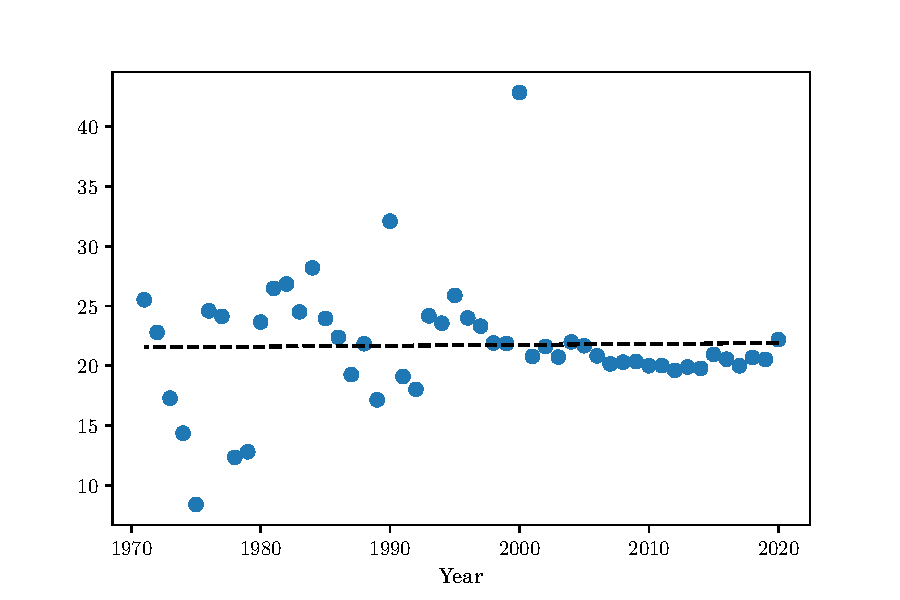
\includegraphics[width=0.9\textwidth]{img/graph-dataset/weekend-work}
    \caption{Ratio of commits performed during the week-end each year plotted
    over time. A linear regression shows a flat trend over a period of fifty
    years.}%
    \label{fig:weekend-work}
\end{figure}


SQL queries can also be used to express more complex tasks.  Consider the
research hypothesis that weekend work on open source projects is decreasing
over the years as evermore development work is done by companies rather than
volunteers.  The corresponding data can be obtained by finding the ratio
between revisions committed on the weekends of each year and the total number
of that year's revisions (see \cref{lst:weekend-work}).
The results, obtained by scanning 14~GiB\ in $7''$, are shown in
\cref{fig:weekend-work}. A linear regression shows that this ratio generally
remained constantly around 22\% over time. These results are inconclusive, and
points to the need for further analysis to validate the hypothesis, which is
left as an exercise to the reader.

\begin{listing}
    \inputminted[firstline=4]{sql}{codesamples/graph-dataset/fork-size.sql}
    \caption{Average number of parents in a revision.}%
    \label{lst:fork-size}
\end{listing}

The provided dataset forms a graph, which can be difficult to query with SQL\@.
Therefore, questions associated with the graph's characteristics,
such as closeness, distance, and centrality, will require the use of
other query mechanisms.
Yet interesting metrics can be readily obtained by limiting scans
to specific cases, such as merge commits.
As an example, \cref{lst:fork-size} calculates the average
number of parents of each revision ($1.088$, after scanning 23~GiB\ in $22''$)
by grouping revisions by their parent identifier.
Such queries can be used to examine in depth the characteristics
of merge operations.

\begin{listing}
    \inputminted[firstline=4]{sql}{codesamples/graph-dataset/file-type-size.sql}
    \caption{Average size of the most popular file types.}%
    \label{lst:file-type-size}
\end{listing}

Although the performance of Athena can be impressive, there are cases where the
available memory resources will be exhausted, causing an expensive query to
fail.
This typically happens when joining two equally large tables consisting of
hundreds of millions of records.
This restriction can be overcome by sampling the corresponding tables.
\Cref{lst:file-type-size} demonstrates such a case.
The objective here is to determine the modularity at the level of files among
diverse programming languages, by examining the size of popular file types.
The query joins two 5~billion row tables:
the file names and the content metadata.
To reduce the number of joined rows a 1\% sample of the rows is processed,
thus scanning 317~GiB\ in $1'20''$.
The order of the resulting language files
(JavaScript $>$ C $>$ C++ $>$ Python $>$ \textsc{php} $>$ C\# $>$ Ruby)
indicates that, with the exception of JavaScript,\footnote{This is likely
    because Javascript is often used as a target format for transcompilation,
    minification and source code bundling.} languages offering more abstraction
    facilities are associated with smaller source code files.

\subsection{Spark on Azure Databricks}

For a more fine-grained control of the computing resources, it is also possible
to use the dataset on Spark, through a local install or using the public
dataset on Azure Databricks. Spark lifts the constraints imposed by limits in
Athena by letting users have a direct control on the number of machines in a
cluster dedicated to their analysis. This offers more flexibility by letting
users choose their own scale factor and the computing power of the nodes in the
cluster.  This is important for computationally intensive experiments or very
large \emph{join} operations, which can only be achieved through sampling in
Athena. One downside of this approach is that it can quickly become rather
expensive, as the cost is no longer solely dependent on the amount of data
analyzed but the real computing resources used while the cluster is running. It
also requires some upfront cost to start the cluster before running any queries
on it.

The dataset is available in a public Azure Data Lake Storage Gen2 container,
and can be loaded directly as temporary views from a Python notebook on Azure
Databricks, as shown in \cref{lst:databricks-load-tables}.
Once the tables are loaded in Spark, the query in
\cref{lst:spark-directory-outdegree} can be used to generate an
out-degree distribution of the directories.

\begin{listing}
\begin{minted}{python}
dataset_path = ('wasbs://swhgraph@swhopendataset.blob.core.windows.net'
                '/2021-03-23/orc')
tables = ['content', 'directory', 'directory_entry', 'origin', 'origin_visit',
          'origin_visit_status', 'release', 'revision', 'revision_history',
          'skipped_content', 'snapshot', 'snapshot_branch']
for table in tables:
    df = spark.read.parquet(dataset_path + '/' + table)
    df.createOrReplaceTempView(table)
\end{minted}
\caption{Load ORC tables in Azure Databricks.}%
\label{lst:databricks-load-tables}
\end{listing}

\begin{listing}
    \inputminted{sql}{codesamples/graph-dataset/spark-degree.sql}
    \caption{Out-degree distribution of directories.}%
    \label{lst:spark-directory-outdegree}
\end{listing}

Spark is flexible in terms of the computations it can perform, thanks to
\glspl{UDF}~\cite{armbrust2015spark} that can be used to specify
arbitrary operations to be performed on the rows.

To analyze the graph structure of the dataset, the GraphFrames
library~\cite{dave2016graphframes} can also be used to perform common
operations on the graph. \Cref{lst:cc} demonstrates how one can load the
edges and nodes of the revision tables as a GraphFrame object, then compute the
distribution of the connected component sizes in this graph. However, running
this experiment on the entire graph can be extremely expensive, as most
distributed graph algorithms require a lot of data synchronization points
between the nodes, and are thus significantly slower than equivalent algorithms
that can run on a single machine. From our own experiments, one should expect a
cost of around \num{5000} USD to compute the connected components of the graph.

\begin{listing}
    \inputminted{python}{codesamples/graph-dataset/spark-cc.py}
    \caption{Connected components of the revision graph.}%
    \label{lst:cc}
\end{listing}
